%-------------------------------------------------------------------------------
% 请勿删除本注释
% Free Response Question 1
%
% 指引:
% 如在小问之前有通用问题描述,请放置于此
%-------------------------------------------------------------------------------

\question
The electric potential in a region of space as a function of position $x$ is given by the equation $V(x)=\alpha x^{2}+\beta x-\gamma$, where $\alpha=2 \mathrm{~V} / \mathrm{m}^{2}, \beta=7 \mathrm{~V} / \mathrm{m}$, and $\gamma=15 \mathrm{~V}$. All nonelectrical forces are negligible. % 请删除并替换本行,与上一行 \question 之间不要留空行

\begin{parts}

%-------------------------------------------------------------------------------
% 请勿删除本注释
% Part (a)
%
% 指引:
% 如在小问之前有通用问题描述,请放置于此
%-------------------------------------------------------------------------------

\part
An electron starts at rest at $x=0$ and travels to $x=20 \mathrm{~m}$. % 请删除并替换本行,与上一行 \part 之间不要留空行
\begin{subparts}
\subpart Calculate the magnitude of the work done on the electron by the electric field during this process. 
\subpart Calculate the speed of the electron at $x=20 \mathrm{~m}$.
\end{subparts}

%-------------------------------------------------------------------------------
% 请勿删除本注释
% Part (b)
%
% 指引:
% 如在小问之前有通用问题描述,请放置于此
%-------------------------------------------------------------------------------

\part
Derive an equation for the $x$-component of the electric field as a function of position $x$. % 请删除并替换本行,与上一行 \part 之间不要留空行

%-------------------------------------------------------------------------------
% 请勿删除本注释
% Part (c)
%
% 指引:
% 如在小问之前有通用问题描述,请放置于此
%-------------------------------------------------------------------------------

\part
       % 请删除并替换本行,与上一行 \part 之间不要留空行
\begin{subparts}
\subpart On the axes below, sketch a graph of the acceleration of the electron $a$ as a function of position $x$.

\begin{figure}[H]
\centering
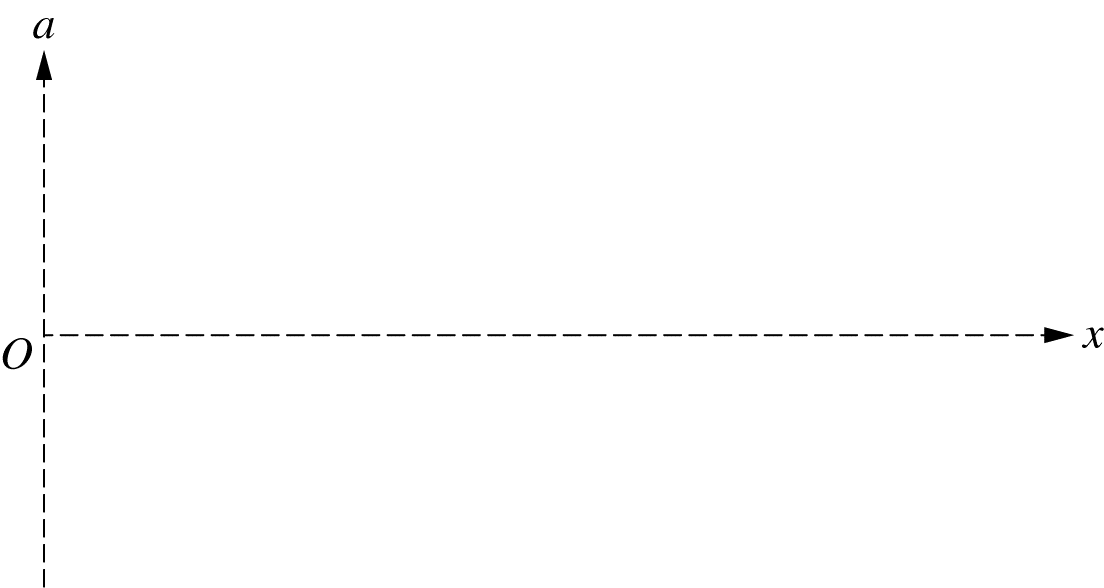
\includegraphics[scale=0.3]{images/img-017-025.png}
\end{figure}

\subpart On the axes below, sketch a graph of the kinetic energy of the electron $K$ as a function of position $x$.

\begin{figure}[H]
\centering
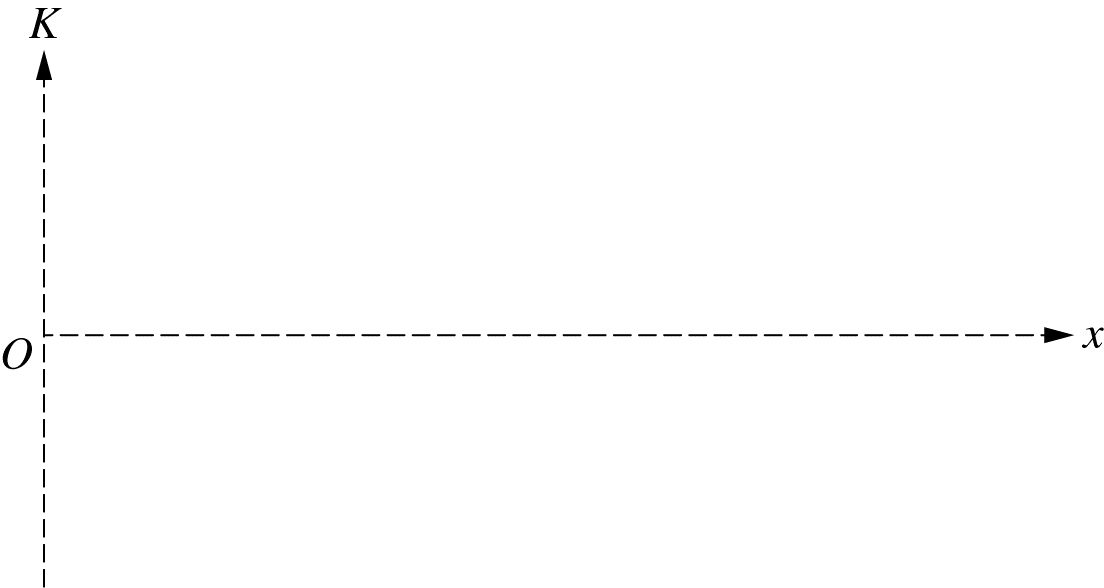
\includegraphics[scale=0.3]{images/img-018-026.png}
\end{figure}

\end{subparts}

%-------------------------------------------------------------------------------
% 请勿删除本注释
% Part (d)
%
% 指引:
% 如在小问之前有通用问题描述,请放置于此
%-------------------------------------------------------------------------------

\part
At which of the following locations will an electron that is released from rest move in the negative $x$ direction? Check all that apply. % 请删除并替换本行,与上一行 \part 之间不要留空行

\underline{\qquad}$x=-2 \mathrm{~m}$ \qquad \underline{\qquad}$x=+1 \mathrm{~m}$\qquad \underline{\qquad}$x=+3 \mathrm{~m}$

Justify your answer.

%-------------------------------------------------------------------------------
% 请勿删除本注释
% Part (e)
%
% 指引:
% 如在小问之前有通用问题描述,请放置于此
%-------------------------------------------------------------------------------

\part
A charged object, generating its own electric field given by $E(x)=7 \mathrm{~V} / \mathrm{m}$, is introduced in the region. What is the potential difference from $x=0 \mathrm{~m}$ to $x=20 \mathrm{~m}$ caused by the combination of the original electrical potential and the electric field of the charged object? % 请删除并替换本行,与上一行 \part 之间不要留空行

\end{parts}
